% Exact model: a_E=5, c=3, a_H=2; X=10/3, Y=4 sqrt(5)/3.
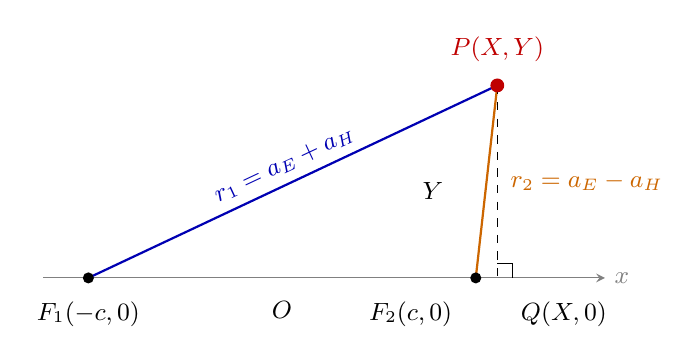
\begin{tikzpicture}[x=.82cm,y=.82cm,>=stealth,font=\small]
\coordinate (L) at (-3,0); \coordinate (R) at (3,0);
\coordinate (P) at (10/3,{4*sqrt(5)/3}); \coordinate (Q) at (10/3,0);
\draw[->,gray] (-3.7,0)--(5,0) node[right] {$x$};
\draw[blue!70!black,thick] (L)--(P) node[midway,above,sloped] {$r_1=a_E+a_H$};
\draw[orange!80!black,thick] (R)--(P) node[midway,right=5pt] {$r_2=a_E-a_H$};
\draw[dashed] (P)--(Q) node[pos=.55,left=16pt] {$Y$};
\draw (10/3,.23)--({10/3+.23},.23)--({10/3+.23},0);
\fill (L) circle (2pt) node[below=5pt] {$F_1(-c,0)$};
\fill (R) circle (2pt) node[below left=5pt] {$F_2(c,0)$};
\fill[red!75!black] (P) circle (2.5pt) node[above=5pt] {$P(X,Y)$};
\node[below right=5pt] at (Q) {$Q(X,0)$};
\node[below=5pt] at (0,0) {$O$};
\end{tikzpicture}
